\chapter{Separazione cellulare su gradiente di ficoll }

\vspace{0.6cm}

\section{Sommario}

\subsection{Scopo}

In questa esperienza introduciamo la metodologia di separazione per le cellule del sangue.
Questa operazione viene effettuata per purificare linfociti e monociti,
separandoli dai globuli rossi e dai granulociti (esempio piastrine) che sono di gran
lunga i componenti più numerosi del sangue.\\
Coinsiderazione: essendo che non possiamo lavorare con il sangue in quanto può
essere molto rischioso abbiamo usato delle cellule di melanoma prese da una coltura.


\subsection{Cenni teorici}
Questa procedura viene usata specialmente per il sangue.
Essa permette di isolare le sue diverse componenti in modo tale da poter successivamente
lavorare più nello specifico con quelle di nostro interesse.\\
Un ruolo importante lo riveste il Ficoll.
Il Ficoll è un copolimero sintetico di alto peso molecolare e grazie alla sua densità
permette di spingere verso il fondo quelle componenti che non ci interessano.
Quindi nel caso del sangue otterremo 4 diverse fasi:
\begin{figure}[H]
    \centering
    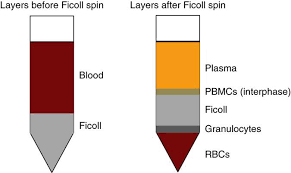
\includegraphics{./immagini/Ficoll_sangue.png}
    \caption{Falcon con sangue pre e post centrifuga}
\end{figure}

\section{Materiali utilizzati}

\begin{itemize}
\item Guanti in lattice
\item Provette Eppendorf (1.5 mL)
\item Falcon da 15 ml
\item Falcon da 50ml
\item Camera di Burker
\item Centrifuga
\item Micropipetta (\SI{100}{\micro\liter}-\SI{1000}{\micro\liter})

\end{itemize}

\section{Soluzioni utilizzate}

\begin{itemize}

\item PBS
\item Tripsina
\item Wash Buffer (terreno di coltura contenente FBS)
\item FBS
\item Ficoll

\end{itemize}

\section{Procedimento}

\subsection{Preparazione della sospensione cellulare}

\begin{enumerate}

    \item Eliminare il terreno di coltura

    \item Lavare le cellule con 20 ml di PBS; eliminare il liquido di lavaggio

    \item Ripetere il lavaggio con ulteriori 20 ml di PBS; eliminarlo

    \item Addizzionare 5 ml di tripsina; lasciare incubare per 5' a 37°C.
    La tripsina permette di staccare le cellule in modo non meccanico (senza cell scraper).

    \item Addizionare alla tripsina 15 ml di Wash Buffer (terreno di coltura con FBS).

    \item Centrifugare a 300g per 10' RT.

    \item Risospendere in 50 ml di Wash Buffer.

    \item A 5 ml di sospensione aggiungere ulteriori 5 ml di Wash Buffer portando
    ad un volume di 10 ml totali.

\end{enumerate}

\subsection{Allestimento separazione su gradiente}

\begin{enumerate}
    \item Diluire il PBS 10X e prelevarne 50 ml 1X in una falcon da 50 ml.
    \item Aliquotare su una Falcon da 15 ml 4 ml di Ficoll.
    \item Stratificare molto lentamente, mediante l'utilizzo di una Pasteur monouso,
    la sospensione di cellule; bisogna far attenzione a non agitare per non compromettere
    la stabilità della deposizione su Ficoll.
    \item Centrifugare per 30' a 800 g RT senza accelerazione nè freno.
    \item Dopo la centrifuga si ottiene una separazione su gradiente che isolerà le cellule
    formando un anello in base alla loro densità. Otteniamo nel nostro caso solo una fase,
    ma nel caso del sangue si vedrebbero diverse fasi che rappresentano le varie componenti.
    \item Prelevare l'anello di cellule formatosi tra il Ficoll e il liquido si sospensione
    cellulare facendo particolare attenzione in quanto è un passaggio delicato.
    Prelevato l'anello spostarlo in una Falcon da 15 ml.
    \item Riempire per decantazione la Falcon di PBS portandolo a un volume finale di 15 ml.
    \item Centrifugare a 400g per 10'; finita la centrifuga scartare il surnatante
    e risospendere il pellet di cellule.
    \item Aggiungere per decantazione ulteriore PBS e portarlo a un volume di 10 ml.
    \item Centrifugare nuovamente a 400 g per 10'; finita la centrifuga scartare di nuovo
    il surnatante e risospendere in 1ml di PBS con la micropipetta da 100 $\mu$.
    \item Spostare infine su una eppendorf da 1.5 ml.
\end{enumerate}

\subsection{Conta cellulare su camera contaglobuli di Burker}
\begin{enumerate}
    \item Diluire le cellule 1:10 in $\mu$ finali su nuova eppendorf.
    \item Montare la camera di Burker.

    \begin{figure}[H]
    \centering
    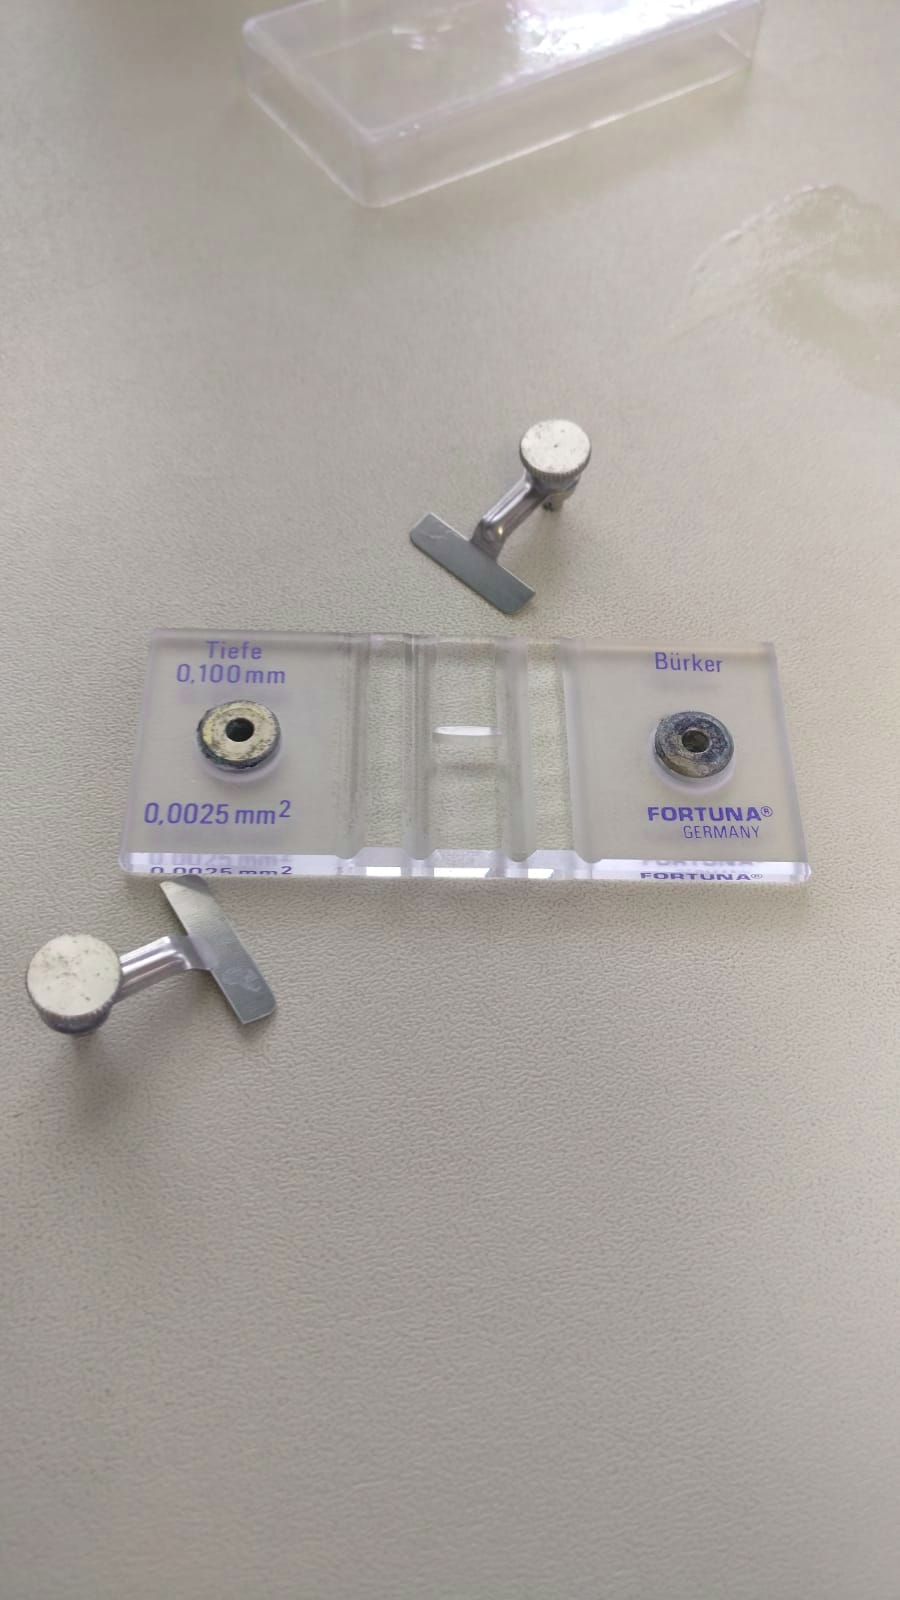
\includegraphics[width = 0.4\textwidth]{./immagini/Burker.png}
    \caption{Burker}
    \end{figure}

    \item Riempire i due pozzetti della camera per capillarità mediante l'utilizzo di
    una pipetta da 200 $\mu$l. Capiamo che la camera è piena quando da sotto il
    copri-vetrino uscirà una goccia.
    \item Contare le cellule comprese all'interno del quadrato che presenta come bordo 3
    righe.
\end{enumerate}

\section{Risultati e Conclusioni}

Il numero di cellule da noi trovate è 92. Un numero così elevato è stato ottenuto per la
non diluizione specificata precedentemente. \\
Il totale delle cellule diluite si sarebbe ottenuto con questa formula :
    $$[cellule] = (num. cellule)*(fatt. diluzione)*(fatt. moltiplicativo camera)$$
Nel nostro caso il fattore moltiplicativo della camerà è 10000.

\end{document}
